\documentclass[12 pt]{beamer}\usepackage[]{graphicx}\usepackage[]{color}
%% maxwidth is the original width if it is less than linewidth
%% otherwise use linewidth (to make sure the graphics do not exceed the margin)
\makeatletter
\def\maxwidth{ %
  \ifdim\Gin@nat@width>\linewidth
    \linewidth
  \else
    \Gin@nat@width
  \fi
}
\makeatother

\definecolor{fgcolor}{rgb}{0.196, 0.196, 0.196}
\newcommand{\hlnum}[1]{\textcolor[rgb]{0.063,0.58,0.627}{#1}}%
\newcommand{\hlstr}[1]{\textcolor[rgb]{0.063,0.58,0.627}{#1}}%
\newcommand{\hlcom}[1]{\textcolor[rgb]{0.588,0.588,0.588}{#1}}%
\newcommand{\hlopt}[1]{\textcolor[rgb]{0.196,0.196,0.196}{#1}}%
\newcommand{\hlstd}[1]{\textcolor[rgb]{0.196,0.196,0.196}{#1}}%
\newcommand{\hlkwa}[1]{\textcolor[rgb]{0.231,0.416,0.784}{#1}}%
\newcommand{\hlkwb}[1]{\textcolor[rgb]{0.627,0,0.314}{#1}}%
\newcommand{\hlkwc}[1]{\textcolor[rgb]{0,0.631,0.314}{#1}}%
\newcommand{\hlkwd}[1]{\textcolor[rgb]{0.78,0.227,0.412}{#1}}%

\usepackage{framed}
\makeatletter
\newenvironment{kframe}{%
 \def\at@end@of@kframe{}%
 \ifinner\ifhmode%
  \def\at@end@of@kframe{\end{minipage}}%
  \begin{minipage}{\columnwidth}%
 \fi\fi%
 \def\FrameCommand##1{\hskip\@totalleftmargin \hskip-\fboxsep
 \colorbox{shadecolor}{##1}\hskip-\fboxsep
     % There is no \\@totalrightmargin, so:
     \hskip-\linewidth \hskip-\@totalleftmargin \hskip\columnwidth}%
 \MakeFramed {\advance\hsize-\width
   \@totalleftmargin\z@ \linewidth\hsize
   \@setminipage}}%
 {\par\unskip\endMakeFramed%
 \at@end@of@kframe}
\makeatother

\definecolor{shadecolor}{rgb}{.97, .97, .97}
\definecolor{messagecolor}{rgb}{0, 0, 0}
\definecolor{warningcolor}{rgb}{1, 0, 1}
\definecolor{errorcolor}{rgb}{1, 0, 0}
\newenvironment{knitrout}{}{} % an empty environment to be redefined in TeX

\usepackage{alltt}

\usepackage{beamerthemesplit}
\usepackage{fancyvrb}
\usepackage[usenames,dvipsnames]{xcolor}


%%%%%%%%%%%%%%%%%%%%%%%%%%%%%%%%%%%%%%%%%%%%%%%%%%%%%%%%%%%%%%%%%%%%%%%%%%%%%%%%%%%%

\mode<presentation> {
  \usetheme{Boadilla}
  \usecolortheme{whale}
  \setbeamercovered{transparent}
}

%%%%%%%%%%%%%%%%%%%%%%%%%%%%%%%%%%%%%%%%%%%%%%%%%%%%%%%%%%%%%%%%%%%%%%%%%%%%%%%%%%%%
%% Custom definitions

\definecolor{darkgreen}{rgb}{0,0.3,0}
\definecolor{darkred}{rgb}{0.6,0.0,0}
\definecolor{darkblue}{rgb}{0,0,0.8}
\definecolor{greyish}{rgb}{0.2,0.2,0.2}

\newcommand{\mxnum}[1]{\texttt{\hlnum{#1}}}%
\newcommand{\mxkwc}[1]{\texttt{\hlkwc{#1}}}%
\newcommand{\mxkwd}[1]{\texttt{\hlkwd{#1}}}%

\newcommand{\pkg}[1]{{\fontseries{b}\selectfont #1}}
\renewcommand{\pkg}[1]{{\color{darkgreen}\texttt{#1}}}

%%%%%%%%%%%%%%%%%%%%%%%%%%%%%%%%%%%%%%%%%%%%%%%%%%%%%%%%%%%%%%%%%%%%%%%%%%%%%%%%%%%%
%%




%%%%%%%%%%%%%%%%%%%%%%%%%%%%%%%%%%%%%%%%%%%%%%%%%%%%%%%%%%%%%%%%%%%%%%%%%%%%%%%%%%%%

\title{\large Nobody Knows What It's Like To Be the Bad Man}
\subtitle{The Development Process for the {\tt{caret}} Package}
% \author{\inst{1} Max Kuhn \and \inst{2} Zachary Deane--Mayer}
% \institute{\inst{1} Pfizer Global R$\&$D \and \inst{2} Cognius }
\author[Subham Kuhn \& Deane--Mayer]
{%
   \texorpdfstring{
        \begin{columns}
            \column{.45\linewidth}
            \centering
            Max Kuhn\\
            Pfizer Global R$\&$D\\
            \href{mailto:max.kuhn@pfizer.com}{max.kuhn@pfizer.com}
            \column{.45\linewidth}
            \centering
            Zachary Deane--Mayer\\
            Cognius\\
            \href{mailto:zach.mayer@gmail.com}{zach.mayer@gmail.com}
        \end{columns}
   }
   {John Doe \& Jane Doe}
}
\date{}

%%%%%%%%%%%%%%%%%%%%%%%%%%%%%%%%%%%%%%%%%%%%%%%%%%%%%%%%%%%%%%%%%%%%%%%%%%%%%%%%%%%%
\IfFileExists{upquote.sty}{\usepackage{upquote}}{}
\begin{document}

\begin{frame}[plain]
  \maketitle
\end{frame}

\title{\tt{caret}}
\author{Kuhn \& Deane--Mayer}
\institute{Pfizer / Cognius}

%%%%%%%%%%%%%%%%%%%%%%%%%%%%%%%%%%%%%%%%%%%%%%%%%%%%%%%%%%%%%%%%%%%%%%

  \begin{frame}[fragile]
\frametitle{Model Function Consistency}

Since there are many modeling packages in R written by different people,
there are inconsistencies in how models are specified and
predictions are created.

\vspace{.15in}

For example, many models have only one method of specifying the model
(e.g. formula method only)


\end{frame}

%%%%%%%%%%%%%%%%%%%%%%%%%%%%%%%%%%%%%%%%%%%%%%%%%%%%%%%%%%%%%%%%%%%%%%

  \begin{frame}[fragile]
\frametitle{Generating Class Probabilities Using Different Packages}

\begin{footnotesize}
\begin{center}
\begin{tabular}{rcl}
{\bf Function} && {\bf {\tt predict} Function Syntax} \\
\hline
 \href{http://cran.r-project.org/web/packages/MASS/index.html}{\pkg{MASS}}\texttt{::}\mxkwd{lda} && {\tt \hlkwd{predict}\hlstd{(obj)}} (no options needed)\\
\pkg{stats}\texttt{:::}\mxkwd{glm} && {\tt \hlkwd{predict}\hlstd{(obj,} \hlkwc{type} \hlstd{=} \hlstr{"response"}\hlstd{)}} \\
\href{http://cran.r-project.org/web/packages/gbm/index.html}{\pkg{gbm}}\texttt{::}\mxkwd{gbm} && {\tt \hlkwd{predict}\hlstd{(obj,} \hlkwc{type} \hlstd{=} \hlstr{"response"}\hlstd{, n.trees)}} \\
\href{http://cran.r-project.org/web/packages/mda/index.html}{\pkg{mda}}\texttt{::}\mxkwd{mda} && {\tt \hlkwd{predict}\hlstd{(obj,} \hlkwc{type} \hlstd{=} \hlstr{"posterior"}\hlstd{)}} \\
\href{http://cran.r-project.org/web/packages/rpart/index.html}{\pkg{rpart}}\texttt{::}\mxkwd{rpart} && {\tt \hlkwd{predict}\hlstd{(obj,} \hlkwc{type} \hlstd{=} \hlstr{"prob"}\hlstd{)}}   \\
\href{http://cran.r-project.org/web/packages/RWeka/index.html}{\pkg{RWeka}}\texttt{::}\mxkwd{Weka} && {\tt \hlkwd{predict}\hlstd{(obj,} \hlkwc{type} \hlstd{=} \hlstr{"probability"}\hlstd{)}}  \\
\href{http://cran.r-project.org/web/packages/caTools/index.html}{\pkg{caTools}}\texttt{::}\mxkwd{LogitBoost}  && {\tt \hlkwd{predict}\hlstd{(obj,} \hlkwc{type} \hlstd{=}  \hlstr{"raw"}\hlstd{, nIter)}} \\
\hline \\
\\
\end{tabular}
\end{center}
\end{footnotesize}
\end{frame}

%%%%%%%%%%%%%%%%%%%%%%%%%%%%%%%%%%%%%%%%%%%%%%%%%%%%%%%%%%%%%%%%%%%%%%

  \begin{frame}[fragile]
\frametitle{The \pkg{caret} Package}

The \href{http://cran.r-project.org/web/packages/caret/index.html}{\pkg{caret}}  package was developed to:
  \begin{itemize}
\item create a unified interface for modeling and prediction
(interfaces to 183 models)
\item streamline model tuning using resampling
\item provide a variety of ``helper'' functions and classes for day--to--day model building tasks
\item increase computational efficiency using parallel processing
\end{itemize}

\vspace{.08in}

First commits within Pfizer: 6/2005, First version on CRAN: 10/2007

\vspace{.06in}

Website: \href{http://topepo.github.io/caret/}{http://topepo.github.io/caret/}

\vspace{.06in}

JSS Paper: \href{http://www.jstatsoft.org/v28/i05/paper}{http://www.jstatsoft.org/v28/i05/paper}

\vspace{.06in}

Model List: \href{http://topepo.github.io/caret/bytag.html}{http://topepo.github.io/caret/bytag.html}

\vspace{.06in}

Many computing sections in APM

\end{frame}

%%%%%%%%%%%%%%%%%%%%%%%%%%%%%%%%%%%%%%%%%%%%%%%%%%%%%%%%%%%%%%%%%%%%%%

  \begin{frame}[fragile]
\frametitle{Package Dependencies}



One thing that makes \pkg{caret} different from most other packages is that it uses code from an abnormally large number ($> 80$) of other packages.

\vspace{.1in}

A refresher:

\begin{itemize}
\item \texttt{Depends}: required for package to function; loaded when \pkg{caret} is loaded
\item \texttt{Imports}: required for package to function; not loaded
\item \texttt{Suggests}: the package uses it sometimes; not loaded
\end{itemize}

\end{frame}


%%%%%%%%%%%%%%%%%%%%%%%%%%%%%%%%%%%%%%%%%%%%%%%%%%%%%%%%%%%%%%%%%%%%%%

\begin{frame}[fragile]
\frametitle{``Simple'"'' Example (38 Nodes)}
\vspace{-.5in}
  \begin{center}
    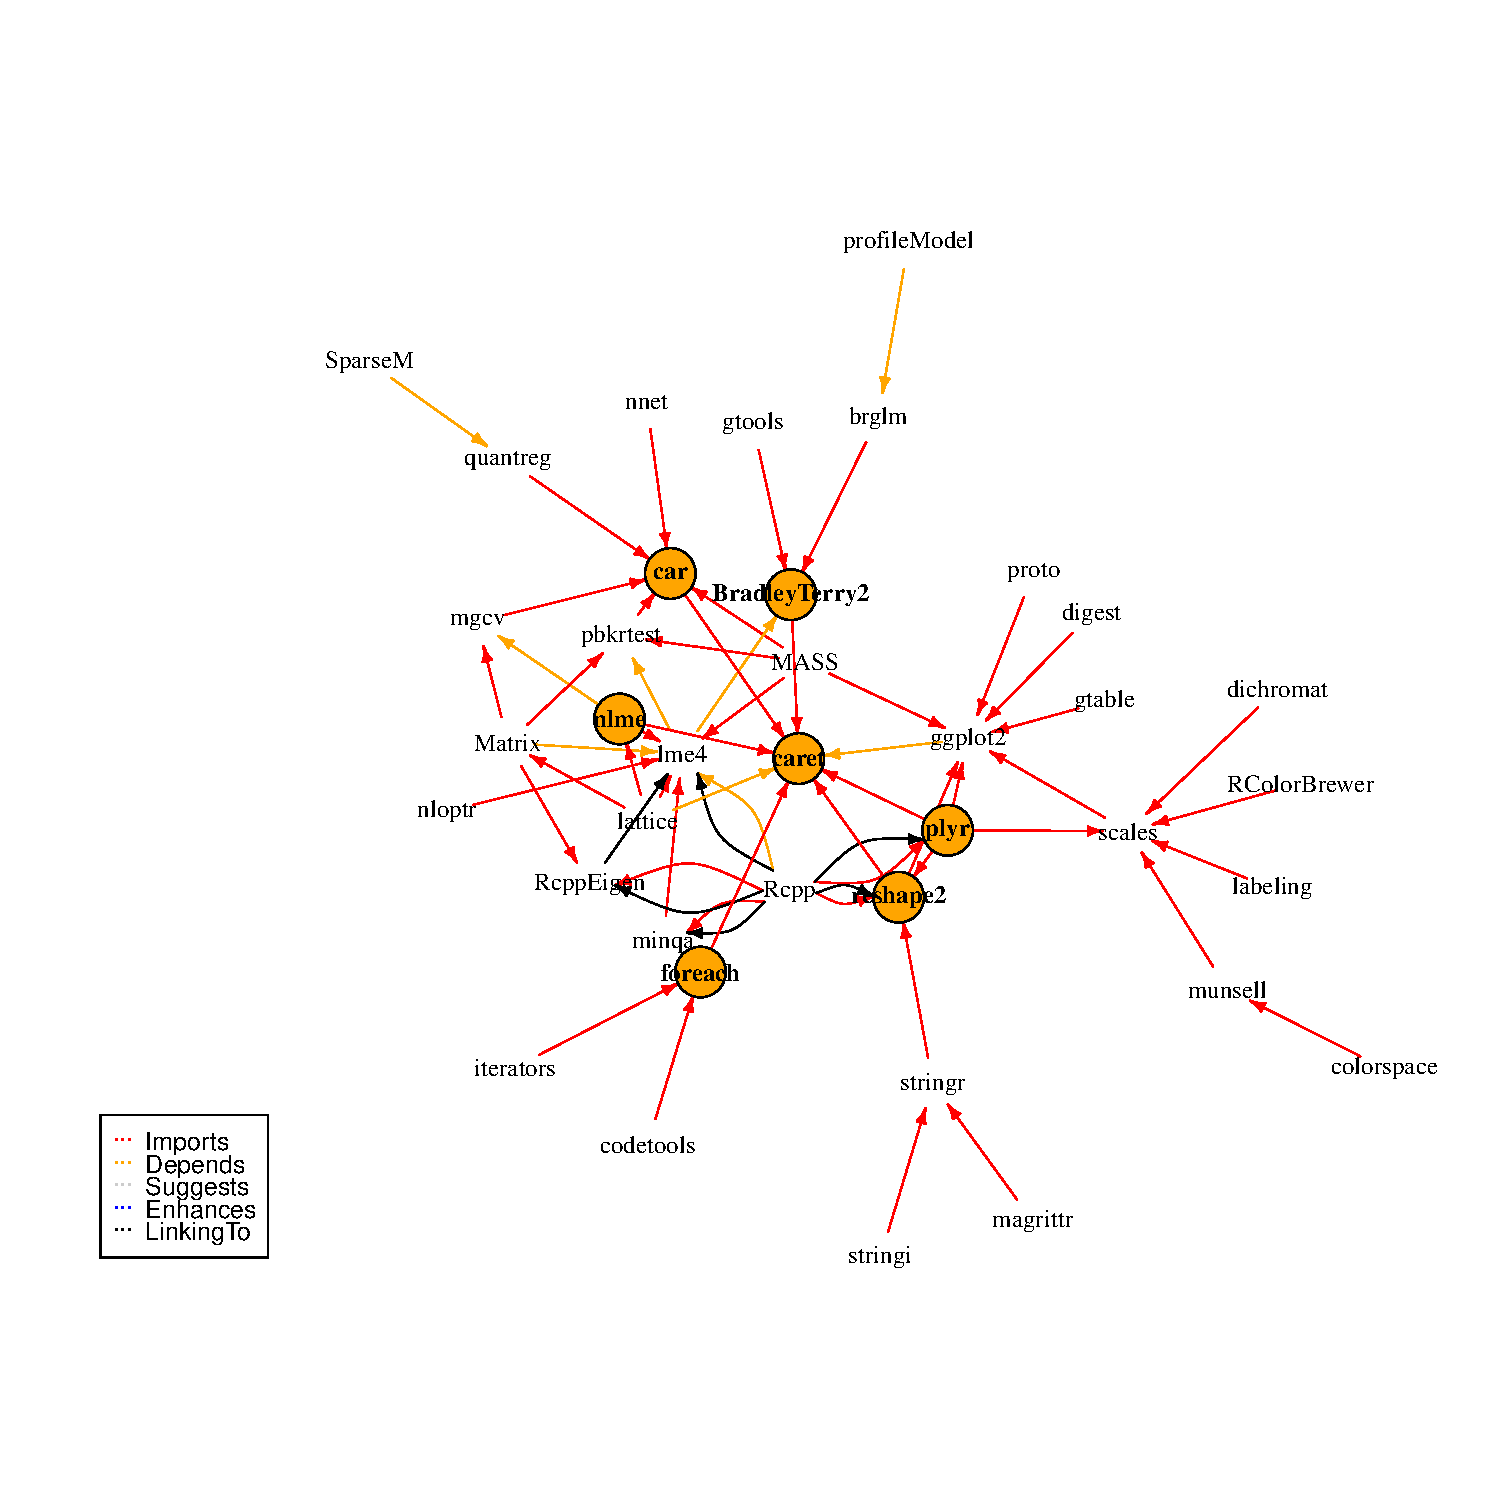
\includegraphics[clip, width = .85\textwidth]{min_graph}
  \end{center}
\end{frame}



%%%%%%%%%%%%%%%%%%%%%%%%%%%%%%%%%%%%%%%%%%%%%%%%%%%%%%%%%%%%%%%%%%%%%%

\begin{frame}[fragile]
\frametitle{Package Dependencies}


Originally, these were in the \texttt{Depends} field of the \textt{DESCRIPTION} file which caused all of them to be loaded with \pkg{caret}.

\vspace{.15in}

For many years, they were moved to \texttt{Suggests}, which solved that issue.


\vspace{.15in}

However, their formal dependency in the \textt{DESCRIPTION} file required CRAN  to install hundreds of other packages to check  \pkg{caret}. The maintainers were not pleased.

\end{frame}



%%%%%%%%%%%%%%%%%%%%%%%%%%%%%%%%%%%%%%%%%%%%%%%%%%%%%%%%%%%%%%%%%%%%%%

  \begin{frame}[fragile]
\frametitle{Package Dependencies in \pkg{caret} Version 5.17-07}
\vspace{-.5in}
  \begin{center}
    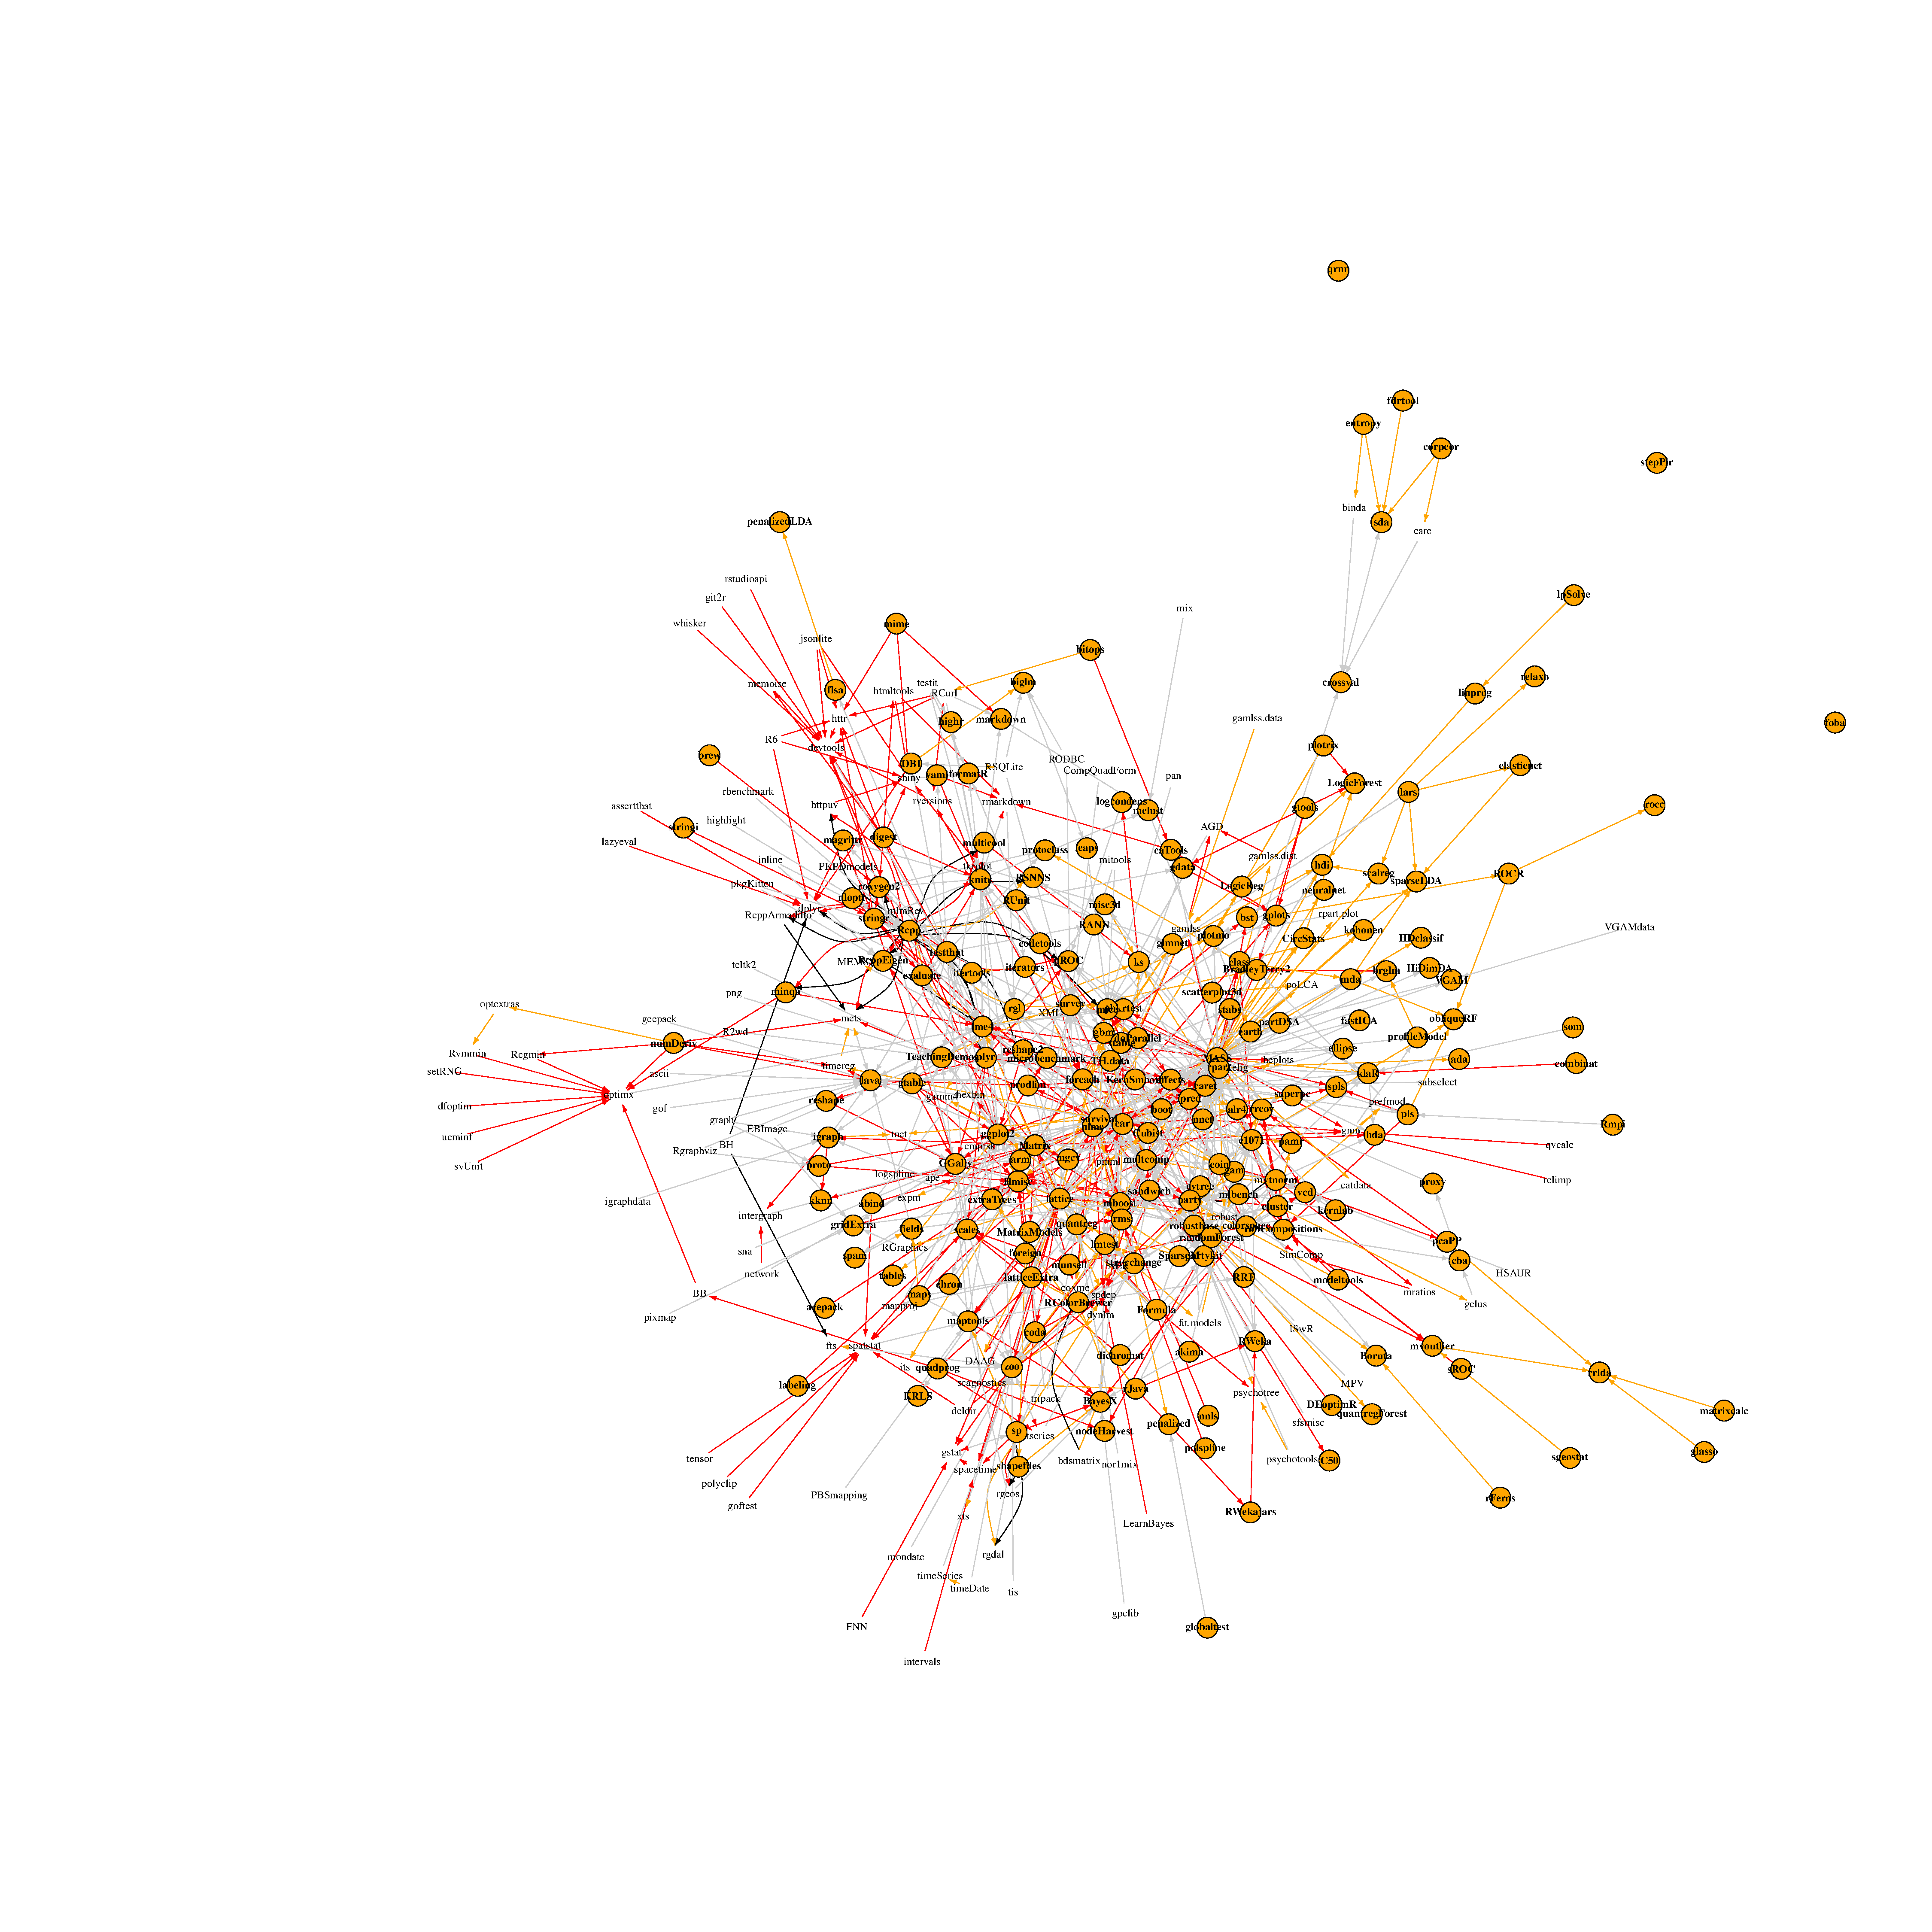
\includegraphics[clip, width = .85\textwidth]{old_graph}
  \end{center}

\end{frame}


%%%%%%%%%%%%%%%%%%%%%%%%%%%%%%%%%%%%%%%%%%%%%%%%%%%%%%%%%%%%%%%%%%%%%%

\begin{frame}[fragile]
\frametitle{Package Dependencies}

This problem was somewhat alleviated at the end of 2013 when {\em custom methods} were expanded.

\vspace{.1in}

Although this functionality had already existed in the package for some time, it was refactored to be more user friendly.

\vspace{.1in}

In the process, much of the modeling code was moved out of \pkg{caret}'s R files and into R objects, eliminating the formal dependencies.

\vspace{.1in}

Right now, the {\em total} number of dependencies is much smaller (2 \texttt{Depends}, 7 \texttt{Imports}, and 25 \texttt{Suggests}).

\vspace{.1in}

This still affects testing though (described later). Also:

\vspace{.1in}

{\tt \color{darkblue} \footnotesize 1 package is needed for this model and is not installed. (gbm). Would you like to try to install it now?}

\end{frame}


%%%%%%%%%%%%%%%%%%%%%%%%%%%%%%%%%%%%%%%%%%%%%%%%%%%%%%%%%%%%%%%%%%%%%%

  \begin{frame}[fragile]
\frametitle{38 Dependencies for \pkg{caret} Version 6.0-47 }
\vspace{-.5in}
  \begin{center}
    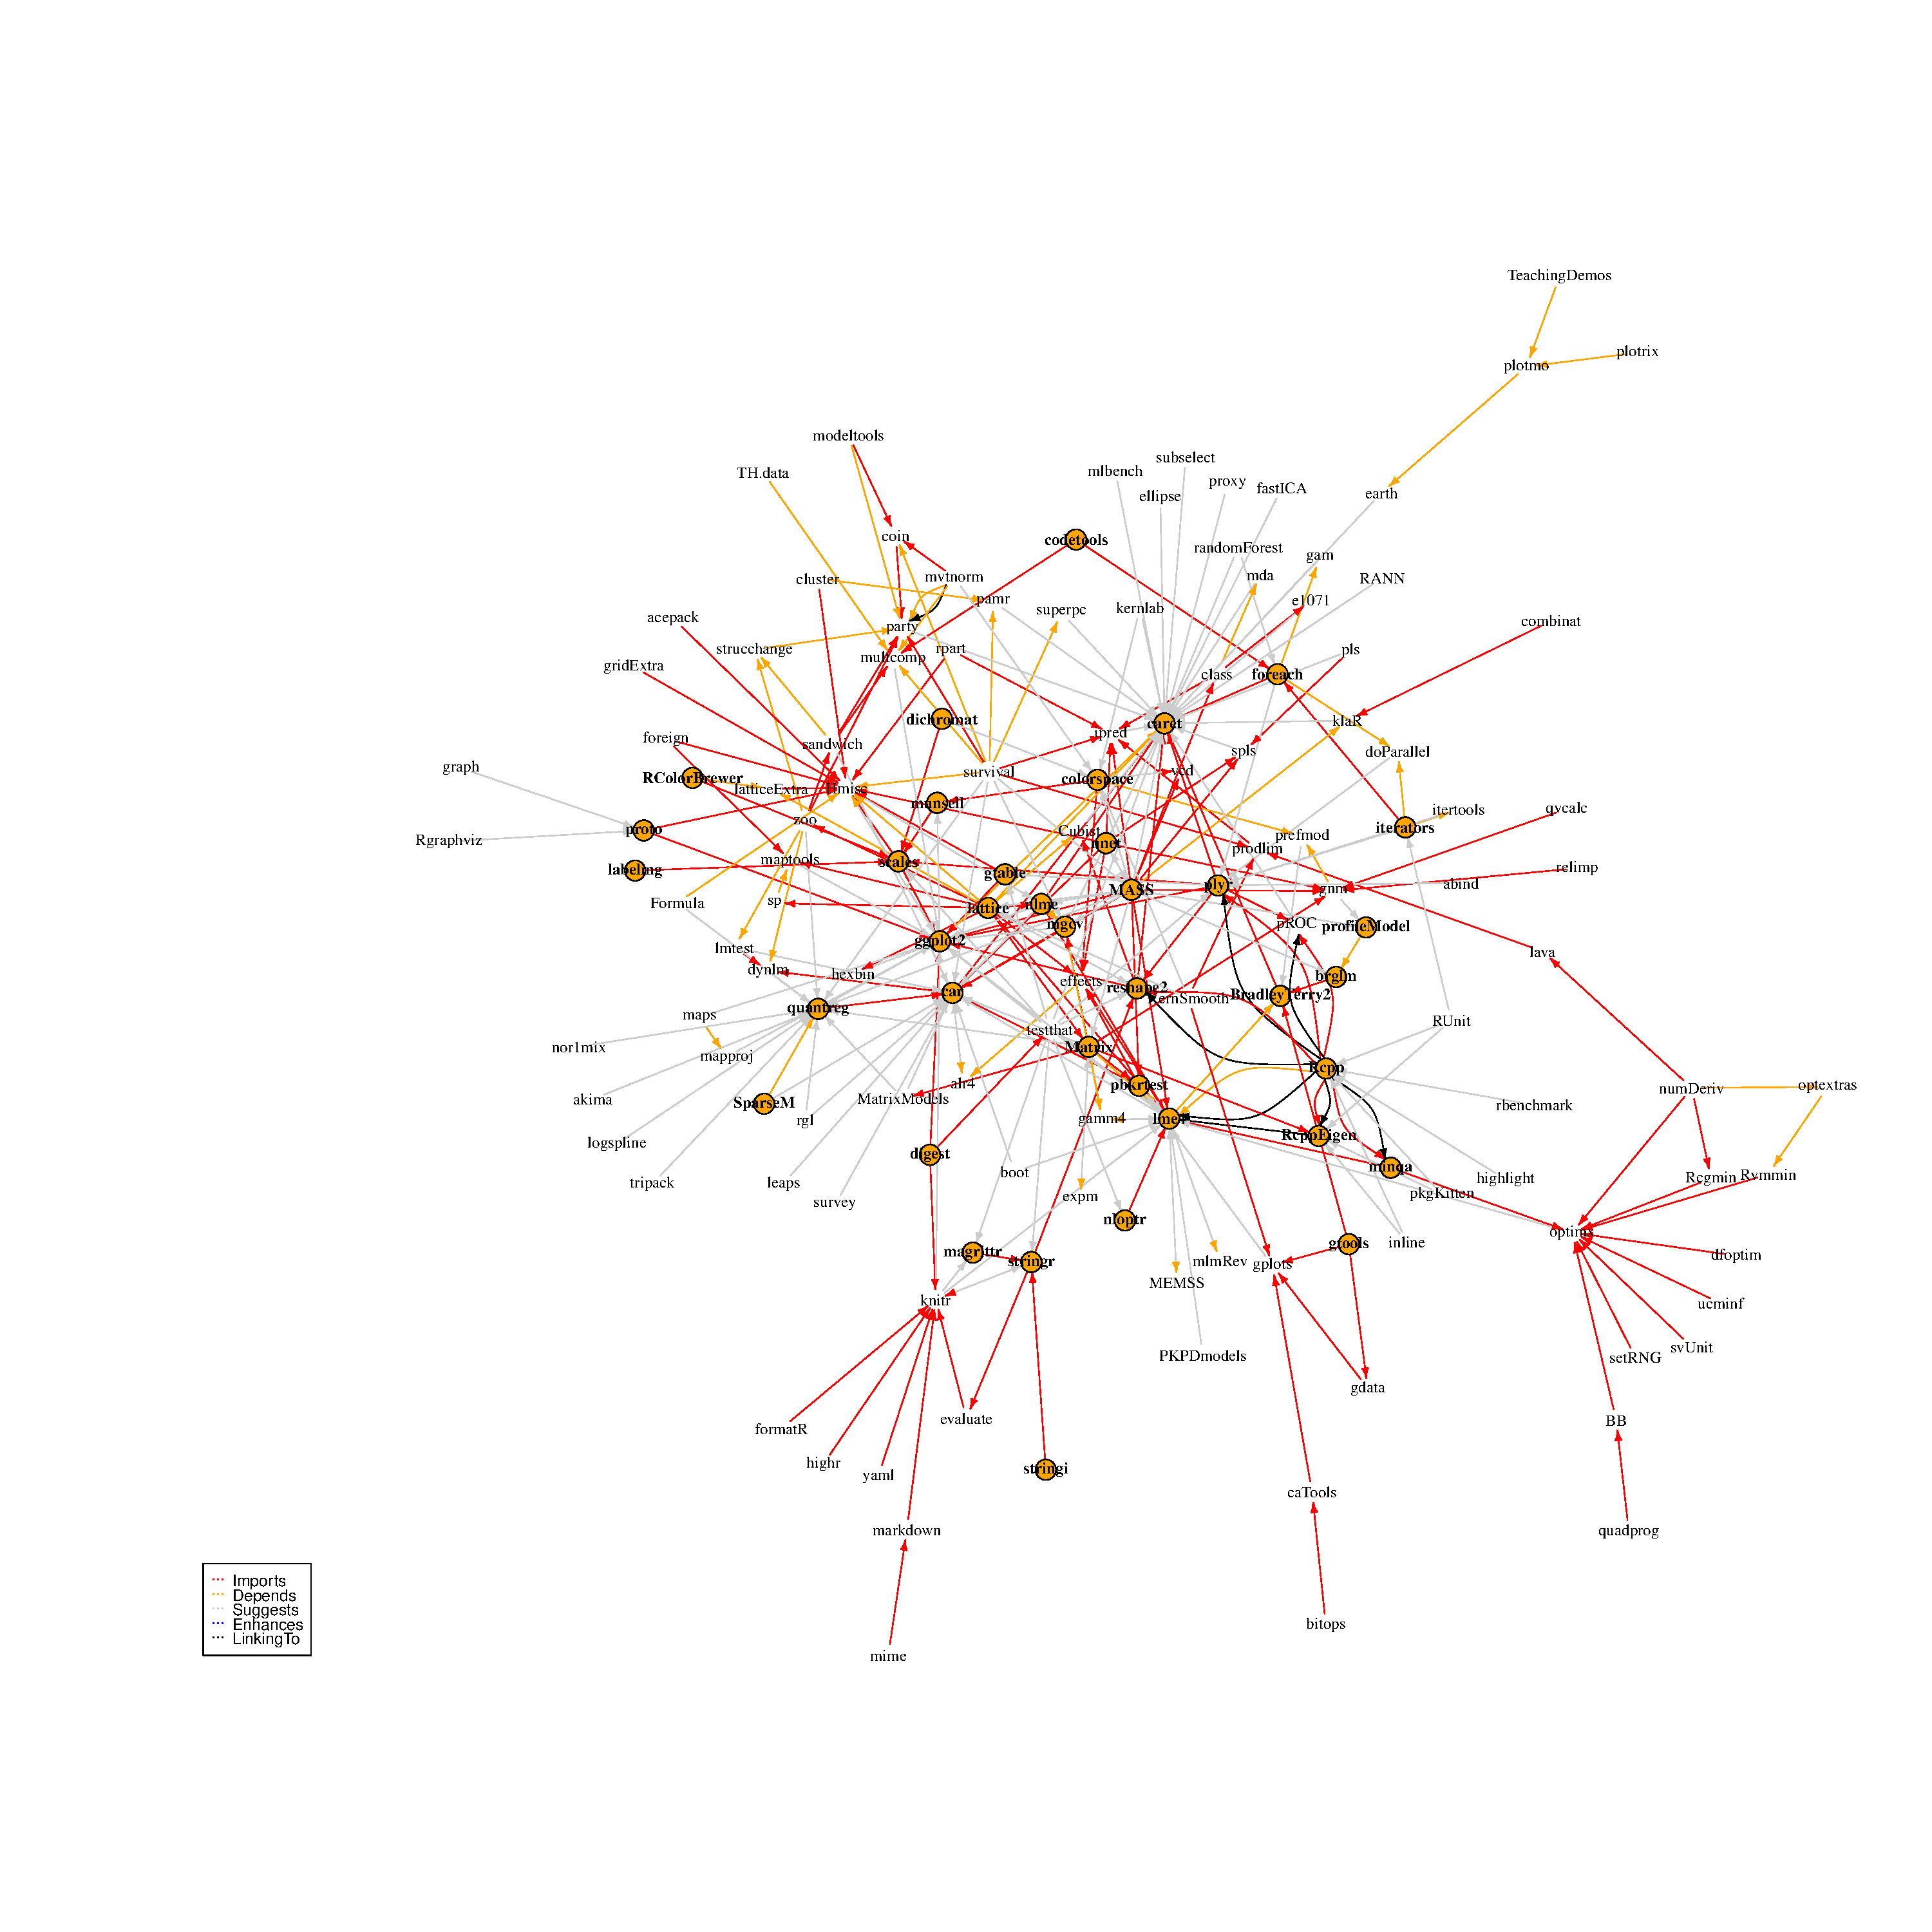
\includegraphics[clip, width = .85\textwidth]{new_graph}
  \end{center}

\end{frame}

%%%%%%%%%%%%%%%%%%%%%%%%%%%%%%%%%%%%%%%%%%%%%%%%%%%%%%%%%%%%%%%%%%%%%%

  \begin{frame}[fragile]
\frametitle{The Basic Release Process}

\begin{enumerate}
  \item create a few dynamic man pages
  \item use {\color{darkred} \texttt{R CMD check --as-cran}} to ensure passing CRAN tests and {\color{darkred} unit tests}
  \item update all packages (and R)
  \item run {\color{darkred} regression tests} and evaluate results
  \item send to CRAN
  \item repeat
  \item repeat
  \item install passed \pkg{caret} version
  \item generate {\color{darkred} HTML documentation} and sync github io branch
  \item profit!
\end{enumerate}

\end{frame}


%%%%%%%%%%%%%%%%%%%%%%%%%%%%%%%%%%%%%%%%%%%%%%%%%%%%%%%%%%%%%%%%%%%%%%

  \begin{frame}[fragile]
\frametitle{Toolbox}

\begin{itemize}
\item RStudio projects: a clean, self contained package development environment
  \begin{itemize}
  \item  No more {\tt setwd('/path/to/some/folder')} in scripts
  \item Keep track of project-wide standards, e.g. code formatting
  \item An RStudio project was the first thing we added after moving the \href{http://cran.r-project.org/web/packages/caret/index.html}{\pkg{caret}} repository to github
  \end{itemize}
\item \href{http://cran.r-project.org/web/packages/devtools/index.html}{\pkg{devtools}}: automate boring tasks
\item \href{http://cran.r-project.org/web/packages/testthat/index.html}{\pkg{testthat}}: automated unit testing
\item \href{http://cran.r-project.org/web/packages/roxygen2/index.html}{\pkg{roxygen2}}: combine source code with documentation
\item github: source control
\end{itemize}


\end{frame}



%%%%%%%%%%%%%%%%%%%%%%%%%%%%%%%%%%%%%%%%%%%%%%%%%%%%%%%%%%%%%%%%%%%%%%

  \begin{frame}[fragile]
\frametitle{\href{http://cran.r-project.org/web/packages/devtools/index.html}{\pkg{devtools}}}

\href{http://cran.r-project.org/web/packages/devtools/index.html}{\pkg{devtools}}{\tt ::\mxkwd{install}} builds package and installs it locally

\vspace{.1in}

\href{http://cran.r-project.org/web/packages/devtools/index.html}{\pkg{devtools}}{\tt ::\mxkwd{check}}:
\begin{enumerate}
  \item  Builds documentation
  \item Runs unit tests
  \item Builds tarball
  \item Runs {\tt R CMD CHECK}
\end{enumerate}

\vspace{.1in}

\href{http://cran.r-project.org/web/packages/devtools/index.html}{\pkg{devtools}}{\tt ::\mxkwd{release}} builds package and submits it to CRAN

\vspace{.1in}

\href{http://cran.r-project.org/web/packages/devtools/index.html}{\pkg{devtools}}{\tt ::\mxkwd{install\_github}} enables non-CRAN code distribution or distribution of private packages

\vspace{.1in}

\href{http://cran.r-project.org/web/packages/devtools/index.html}{\pkg{devtools}}{\tt ::\mxkwd{use\_travis}} enables automated unit testing through travis-CI and test coverage reports through coveralls

\end{frame}




%%%%%%%%%%%%%%%%%%%%%%%%%%%%%%%%%%%%%%%%%%%%%%%%%%%%%%%%%%%%%%%%%%%%%%

  \begin{frame}[fragile]
\frametitle{Testing}

Testing for the package occurs in a few different ways:
\begin{itemize}
\item units tests via \href{http://cran.r-project.org/web/packages/testthat/index.html}{\pkg{testthat}} and travis-CI
\item regression tests for consistency
\end{itemize}

\vspace{.2in}

Automated unit testing via \href{http://cran.r-project.org/web/packages/testthat/index.html}{\pkg{testthat}}

\begin{itemize}
\item \href{http://cran.r-project.org/web/packages/testthat/index.html}{\pkg{devtools}}{\tt ::\mxkwd{use\_testhat}}
\item Unit tests prevent new features from breaking old code
\item All functions should have associated tests
\item Run during {\tt R CMD check --as-cran}
\item Can specify that certain tests be skipped on CRAN
\end{itemize}

\href{http://cran.r-project.org/web/packages/caret/index.html}{\pkg{caret}} is slowly adding more \href{http://cran.r-project.org/web/packages/testthat/index.html}{\pkg{testthat}} tests

\end{frame}

%%%%%%%%%%%%%%%%%%%%%%%%%%%%%%%%%%%%%%%%%%%%%%%%%%%%%%%%%%%%%%%%%%%%%%

  \begin{frame}[fragile]
\frametitle{github + travis + coveralls}

Travis and coveralls are tools for automated unit testing
\begin{itemize}
\item Travis reports test failutes and CRAN errors/warnings
\item Coveralls reports \% of code covered by unit tests
\item Both automatically comment on the PR itself
\end{itemize}

\vspace{.1in}

Contributor submits code via a pull request

\begin{itemize}
\item Travis notifies them of test failures
\item Coveralls notifies them to write tests for new functions
\item Automated feedback on code quality allows rapid iteration
\end{itemize}

\vspace{.1in}

Code review once unit tests and R CMD CHECK pass
\begin{itemize}
\item github supports line-by-line comments
\item Usually several more iterations here
\end{itemize}

\end{frame}

%%%%%%%%%%%%%%%%%%%%%%%%%%%%%%%%%%%%%%%%%%%%%%%%%%%%%%%%%%%%%%%%%%%%%%

\begin{frame}[fragile]
\frametitle{Writing new unit tests}

\begin{itemize}
\item Coveralls identifies un-tested code:
\includegraphics[width=0.15\textwidth]{coverage_12.png}
\item Developer chooses a file with low or no coverage
\item Developer writes unit tests
\end{itemize}
\begin{Verbatim}[fontsize=\footnotesize]
context('Test Data Splitting Functions')
test_that('createTimeSlices', {
  y <- 1:10
  s1 <- createTimeSlices(y, initialWindow=5, horizon=1)
  expect_equal(length(s1$train), 5)
  expect_equal(s1$train$Training1, 1:5)
  expect_equal(s1$test$Testing1, 6)
})
\end{Verbatim}
\begin{itemize}
\item while(coverage\textless 100\%)\{repeat\}
\end{itemize}
\end{frame}

%%%%%%%%%%%%%%%%%%%%%%%%%%%%%%%%%%%%%%%%%%%%%%%%%%%%%%%%%%%%%%%%%%%%%%

  \begin{frame}[fragile]
\frametitle{Regression Testing}

Prior to CRAN release (or whenever required), a comprehensive set of regression tests can be  conducted.

\vspace{.1in}

All modeling packages are updated to their current CRAN versions.

\vspace{.1in}

For each model accessed by \mxkwd{train}, \mxkwd{rfe}, and/or \mxkwd{sbf}, a set of test cases are computed with the production version of \pkg{caret} and the devel version.

\vspace{.1in}

First, test cases are evaluated to make sure that nothing has been broken by updated versions of the consistuent packages.

\vspace{.1in}

Diffs of the model results are computed to assess any differences in \pkg{caret} versions.

\vspace{.1in}

This process takes approximately 3hrs to complete using \texttt{make -j 12} on a Mac Pro.

\end{frame}


%%%%%%%%%%%%%%%%%%%%%%%%%%%%%%%%%%%%%%%%%%%%%%%%%%%%%%%%%%%%%%%%%%%%%%

  \begin{frame}[fragile]
\frametitle{Regression Testing}

\begin{Verbatim}[fontsize=\footnotesize]
$ R CMD BATCH move_files.R
$ cd ~/tmp/2015_04_19_09__6.0-41/
$ make -j 12 -i
 2015-04-19 09:13:44: Starting ada
 2015-04-19 09:13:44: Starting AdaBag
 2015-04-19 09:13:44: Starting AdaBoost.M1
 2015-04-19 09:13:44: Starting ANFIS
                :
 make: [FH.GBML.RData] Error 1 (ignored)
                :
 2015-04-19 12:03:52: Finished WM
 2015-04-19 12:04:48: Finished xyf
\end{Verbatim}

\end{frame}



%%%%%%%%%%%%%%%%%%%%%%%%%%%%%%%%%%%%%%%%%%%%%%%%%%%%%%%%%%%%%%%%%%%%%%

  \begin{frame}[fragile]
\frametitle{Documentation}

\pkg{caret} originally contained four package vignettes with in--depth descriptions of functionality with examples.

\vspace{.15in}

However, this added time to \texttt{R CMD check} and was a general pain for CRAN.

\vspace{.15in}

Efforts to make the vignettes more computationally efficient (e.g. reducing the number of examples, resamples, etc.) diminished the effectiveness of the documentation.


\end{frame}

%%%%%%%%%%%%%%%%%%%%%%%%%%%%%%%%%%%%%%%%%%%%%%%%%%%%%%%%%%%%%%%%%%%%%%

  \begin{frame}[fragile]
\frametitle{Documentation}

The documentation was moved out of the package and to the github IO page.

\vspace{.15in}


These pages are built using \pkg{knitr} whenever a new version is sent to CRAN. Some advantages are:

\begin{itemize}
\item longer and more relevant examples are available
\item update schedule is under my control
\item dynamic documentation (e.g. D3 network graphs, JS tables)
\item better formatting
\end{itemize}

\vspace{.1in}

It currently takes about 4hr to create these (using parallel processing when possible).

\end{frame}



%%%%%%%%%%%%%%%%%%%%%%%%%%%%%%%%%%%%%%%%%%%%%%%%%%%%%%%%%%%%%%%%%%%%%%

\begin{frame}[plain]
\begin{center}
\LARGE Backup Slides
\end{center}
\end{frame}


%%%%%%%%%%%%%%%%%%%%%%%%%%%%%%%%%%%%%%%%%%%%%%%%%%%%%%%%%%%%%%%%%%%%%%

  \begin{frame}[fragile]
\frametitle{\href{http://cran.r-project.org/web/packages/roxygen2/index.html}{\pkg{roxygen2}}}

Simplified package documentation

\vspace{.2in}

Automates many parts of the documentation process
\begin{itemize}
\item  Special comment block above each function
\item Name, description, arguments, etc.
\item Code and documentation are in the same source file
\end{itemize}

\vspace{.2in}

A must have for new packages but hard to convert existing packages
\begin{itemize}
\item   \href{http://cran.r-project.org/web/packages/caret/index.html}{\pkg{caret}} has 92 .Rd files
\item I'm not in a hurry to re-write them all in \href{http://cran.r-project.org/web/packages/roxygen2/index.html}{\pkg{roxygen2}} format
\end{itemize}




\end{frame}




%%%%%%%%%%%%%%%%%%%%%%%%%%%%%%%%%%%%%%%%%%%%%%%%%%%%%%%%%%%%%%%%%%%%%%

  \begin{frame}[fragile]
\frametitle{Required ``Optimizations''}


For example, there is one check that produces a large number of false positive warnings. For example:

\begin{knitrout}\scriptsize
\definecolor{shadecolor}{rgb}{1, 1, 1}\color{fgcolor}\begin{kframe}
\begin{alltt}
\hlstd{> }\hlstd{bwplot.diff.resamples} \hlkwb{<-} \hlkwa{function} \hlstd{(}\hlkwc{x}\hlstd{,} \hlkwc{data}\hlstd{,} \hlkwc{metric} \hlstd{= x}\hlopt{$}\hlstd{metric,} \hlkwc{...}\hlstd{)  \{}
\hlstd{+ }    \hlcom{## some code}
\hlstd{+ }    \hlstd{plotData} \hlkwb{<-} \hlkwd{subset}\hlstd{(plotData, Metric} \hlopt \hlstd{metric)}
\hlstd{+ }    \hlcom{## more code}
\hlstd{+ }\hlstd{\}}
\end{alltt}
\end{kframe}
\end{knitrout}

will trigger a warning that ``{\tt \small bwplot.diff.resamples: no visible binding for global variable 'Metric'}''.

\vspace{.15in}

The ``solution'' is to have a file that is sourced first in the package (e.g. \texttt{aaa.R}) with the line

\begin{knitrout}\scriptsize
\definecolor{shadecolor}{rgb}{1, 1, 1}\color{fgcolor}\begin{kframe}
\begin{alltt}
\hlstd{> }\hlstd{Metric} \hlkwb{<-} \hlkwa{NULL}
\end{alltt}
\end{kframe}
\end{knitrout}

\end{frame}



%%%%%%%%%%%%%%%%%%%%%%%%%%%%%%%%%%%%%%%%%%%%%%%%%%%%%%%%%%%%%%%%%%%%%%

\begin{frame}[fragile]
\frametitle{Judging the Severity of Problems}

It's hard to tell which warnings should be ignored and which should not. There is also the issue of inconsistencies related to who is ``on duty'' when you submit your package.

\vspace{.1in}

It is hard to believe that someone took the time for this:

\vspace{.15in}
\begin{footnotesize}
Description Field: {\tt "My awesome R package"}

{\tt R CMD check: "{\color{red}Malformed Description field: should contain one or more complete sentences.}"}

\vspace{.15in}

Description Field: {\tt "This package is awesome"}

{\tt R CMD check: "{\color{red}The Description field should not start with the package name, 'This package' or similar.}"}

\vspace{.15in}

Description Field: {\tt "Blah blah blah."}

{\tt R CMD check: {\color{green}\bf PASS}}
\end{footnotesize}

\end{frame}



\end{document}

